\documentclass{article}
\setlength{\parindent}{0cm}

@(vfl) = **Vanilla Flavored LaTex**

@(github_url) = http://github.com/adhithyan15/vanilla

@(tmaker) = **TexMaker**

@(ftb) = formatted text blocks

#(cftb)[] = [$(cap)[formatted text blocks]]

$(importpack)[documentation]

\begin{document}

\begin{center}

\huge{Vanilla Documentation}\vspace{5pt}

\large{**Everything that you need to know about Vanilla**}

\end{center}

\vspace{30pt}

\section*{Copyright}

**\textcopyright Adhithya Rajasekaran, Renuka Rajasekaran, Sri Madhavi Rajasekaran**. All the contents in this document are released under a *[creative commons license =>  http://creativecommons.org/licenses/by-nd/3.0/]. 

\section*{What is Vanilla?}

Vanilla is a powerful LaTex preprocessor. It works based on the DRY(Don't Repeat Yourself) principle. It aims to reduce the entry barrier and the learning curve for Latex by simplifying the syntax and also reducing the verbosity of Latex. In this documentation you will learn how to write @(vfl) documents. This document itself is written in @(vfl) \vspace{5pt}

\section*{Why Vanilla?}

LaTex is a wonderful typesetting system but its reach is limited because of its complexity, verbose syntax and steep learning curve. So @(vfl) is directed towards solving those above mentioned problems. It derives most of its ideas from 
**Markdown**, a small but powerful markup language. 

\section*{Open Source Project}

The authors of this project have decided to open source the source code of the project. The code is hosted on *[github => https://github.com/adhithyan15/vanilla]. The code is released under MIT License. Please report any bugs to the *[issues => https://github.com/adhithyan15/vanilla/issues?state=open] tab on our github homepage. If you have any new ideas or suggestions, please leave them on the issues tab. We will greatly appreciate your feedback.   

\section*{Technical Details}

Vanilla first started out as a separate markup language with a backward compatiblity to Latex. But it became apparent that there will be not enough interest in creating large amounts of libraries and productivity tools for Vanilla alone. So the authors departed from the idea and made it a preprocessor that incorporated a lot of features from their original markup language idea. \vspace{5pt}

Any LaTex document is a valid @(vfl) document but no @(vfl) document is a valid LaTex document without being processed through the Vanilla. \vspace{5pt}

The original compiler prototype was built using Matlab and then Python for more reachability. The preprocessor grew out of that compiler and was rewritten from scratch in Ruby and is shipped as a commandline utility.\vspace{5pt}

Vanilla builds on top of **PDFLatex**. So it is very important that you have any of the major tex distributions installed on your computer. If you are on windows I recommend *[MikTex => www.miktex.org] and on mac, I recommend *[MacTex => http://tug.org/mactex/]. \vspace{5pt}

\section*{Current State}

The current and stable vanilla release is version 1.0. The release provides a minimal set of base features which might be retained in most of the future releases. Significant amounts of features have been left out either due to bugs or incomplete implementation or not enough testing. They will be released in the upcoming releases. One of the main drawbacks of Vanilla is that it doesn't ship with an **error catcher and notifier**.  So Vanilla will simply ignore the errors and try to compile the error free parts of the document.\vspace{5pt}

\section*{Getting Vanilla}

It is very easy to get Vanilla. Visit www.adhithyan15.github.com/vanilla/ and follow the steps below. 

\begin{enumerate}

\item Click on "Download Zip" to download both the source of the compiler and also the compiled version of the compiler. \vspace{5pt}

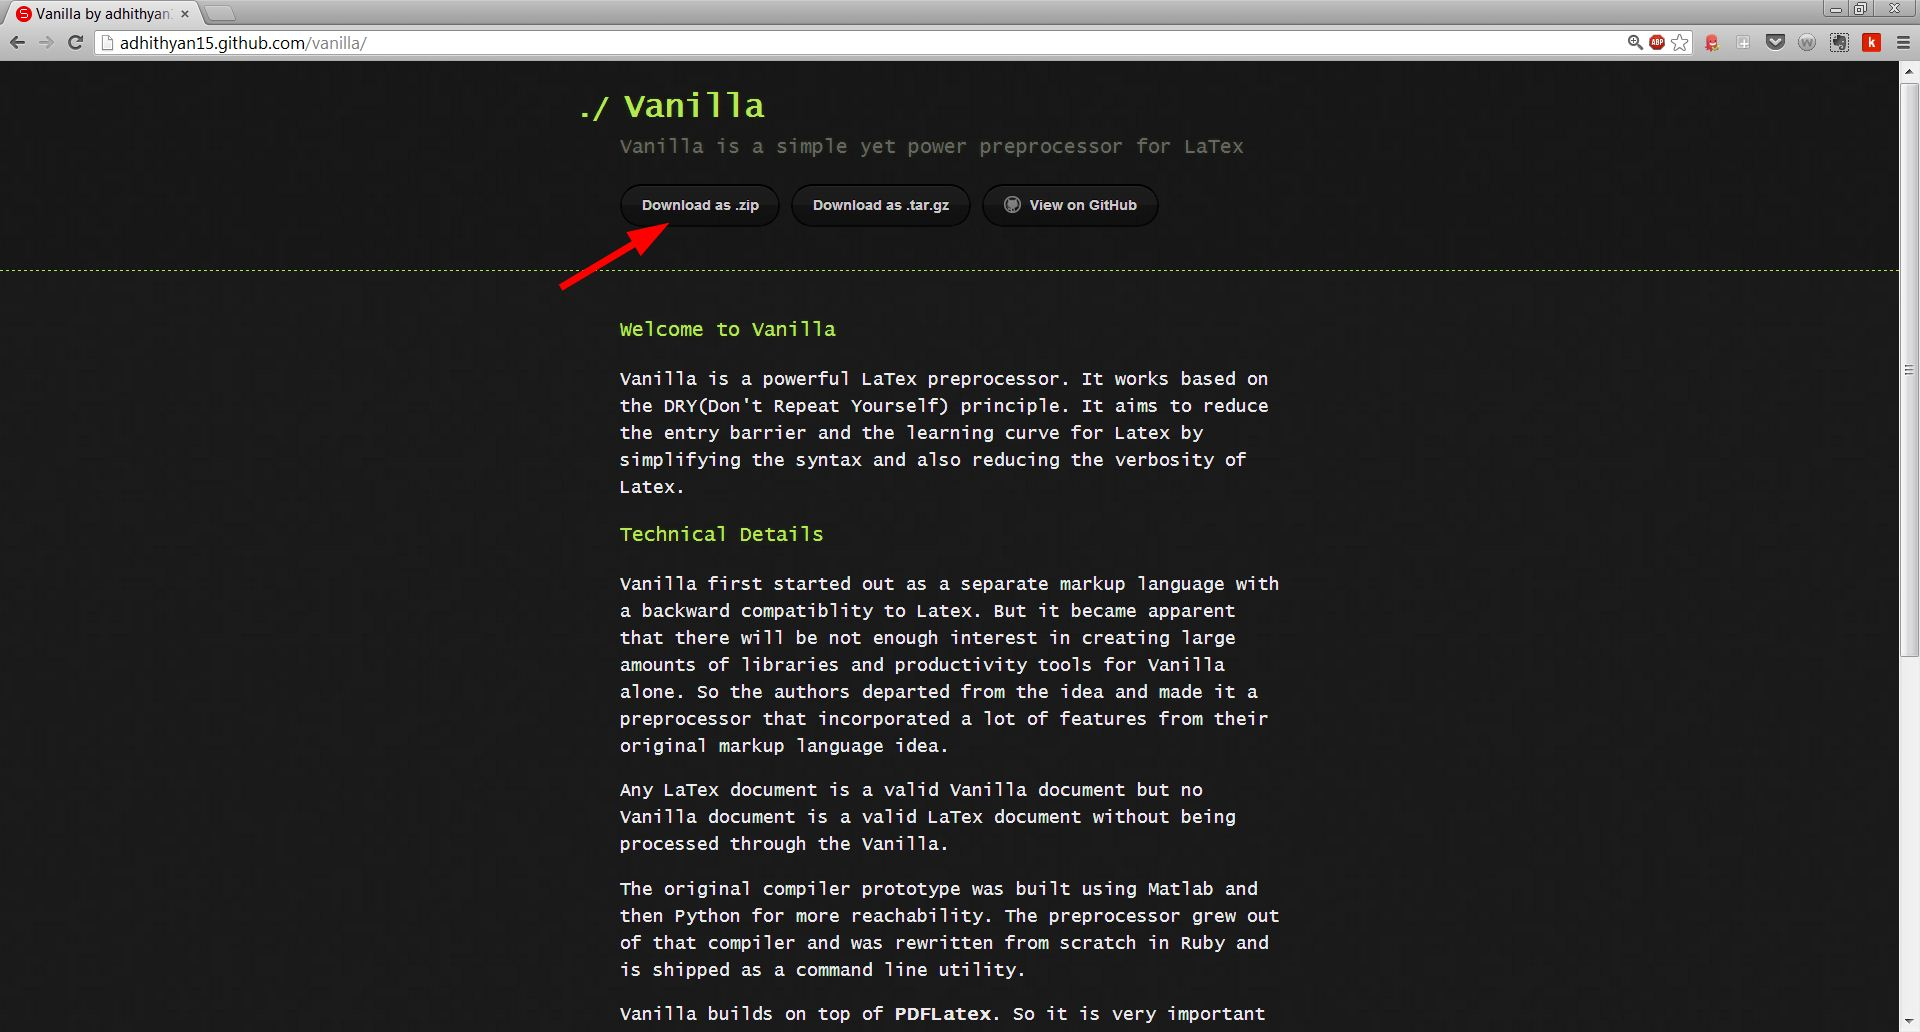
\includegraphics[scale = 0.35]{VanillaGithub}

\item Extract the downloaded zip file using Winzip or any other archive extractor. If you don't have an archive extractor, I recommend *[ 7-zip => www.7zip.org ]

\item Once you extract it, you will find the following files inside the folder you extracted

\begin{itemize}

\item **bin**: The bin directory contains **Vanilla.exe**,**Vanilla**,and **Vanilla.rb** files. **Vanilla.exe** is the primary compiler for the windows platform and **Vanilla** is the primary compiler for the unix platform. **Vanilla.rb** file contains the ruby source code of the compiler. 
\item **Old Compiler Prototypes**: This directory contains the prototype compilers written in Python and Matlab. Those have been open sourced just for reference purposes. 
\item **Readme.md**: Since the project is hosted in *[ Github => @(github_url) ], Github added a readme file markuped in **Markdown**.
\item **VanillaGithub.jpg**: A screenshot of http://adhithyan15.github.com/vanilla page. 
\item **Documentation.pdf**: This is the same document that you are reading right now. 
\item **Documentation.tex**: This is the .tex version of documentation written using @(vfl). I highly recommend you to read through this document so that you can get example usages of @(vfl). 

\end{itemize}

\item For windows users, please follow *[this => https://github.com/adhithyan15/vanilla/wiki/Adding-Vanilla-to-Path] tutorial to add the Vanilla.exe to your path so that it can be accessed from your commandline prompt. Mac and other Unix based OS please follow *[this => https://github.com/adhithyan15/vanilla/wiki/Getting-Started-With-Vanilla-Mac-and-Unix] tutorial to add the utility to your terminal/bash. 

\item You are all set. You can compile your @(vfl) documents by calling **"vanilla --compile somefile.tex"**. You have to set the directory in which your @(vfl) document is located as your **current directory** for the above command to work.

Please see *[this => https://github.com/adhithyan15/vanilla/wiki/Compiling-Vanilla-Flavored-LaTex-Documents] tutorial to understand what the above phrase is describing.    
 
\end{enumerate}

Vanilla compiler can work with LaTex Editors. But configuration seems to be a problem. Vanilla is an unconventional preprocessor in which it doesn't have a seperate extension. After the preprocessing stage, Vanilla needs the authority to overwrite the original file and many of the LaTex editors block that kind of action from happening. So a solution is under development. Until such time, you can use Notepad, Notepad++, Wordpad or Sublime Text. 

\section*{Features of Vanilla}

@(vfl) offers a lot of features to enhance people's productivity with LaTex. Let us see what those features below

\begin{itemize}

\item **Multiline Comments**: In @(vfl) you can comment out multiple lines of code using matlab style comments. Let us see a quick demo of this feature

###

%You can comment out multiple lines using matlab style comments %{.....}%

%{Lorem ipsum dolor sit amet, consectetur adipiscing elit. Mauris placerat tristique purus, 
non tempus mi ultrices in. Praesent lobortis erat et lorem commodo mollis. Pellentesque 
eu euismod nulla.Ut vitae consequat est. Quisque adipiscing rhoncus tellus, eu fermentum 
augue tincidunt ut. Proin a dui dignissim massa auctor iaculis dictum a purus. Suspendisse 
porta felis at velit placerat varius.}%

###

Vanilla compiler converts @(vfl) multiline comments into several single line LaTex comments. Vanilla compiler doesn't touch the LaTex comments. So they are still valid. 

\item **Constants**: Constants are very similar to variables but they are immutable. In @(vfl), you can declare constants
through the following sytax $@(constant\_name) = value$. Note: LaTex has offers mutable variables. We are working on implementing mutable variables in Vanilla. It will be released in
version 2.0. 

###

@(vfl) = **Vanilla Flavored LaTex** %must be declared in the preamble

%Usage

Welcome to @(vfl) %should output Welcome to \textbf{Vanilla Flavored LaTex} 

###

Vanilla compiler doesn't compile the Vanilla constants into LaTex variables. Instead, it converts them into plain text so that they can be used in a variety of purposes.  
Since the constants are rendered into plain text all the you can pass in a variable to most of the features listed below. 

\item **Formatted Text Blocks**: #(cftb)[] were inspired by Less CSS' parametric mixins. #(cftb)[] can include any kind of LaTex or @(vfl) formatting. 
@(vfl) forces the @(ftb) to be declared inside preamble to increase readability and @(ftb) are immutable. Mutable @(ftb) are under development and they will be released in version 2.0. 

###

%Declaration

#(welcome_message)[@(name),@(message)] = [Welcome **@(name)**,@(message)] %should be 
%declared in the preamble

%Usage

#(welcome_message)[Adhithya Rajasekaran,Hello World] %This should output 
%Welcome \textbf{Adhithya Rajasekaran}, Hello World

###

#(cftb)[] can span multiple lines. Parameterless @(ftb) can be used as a constants spanning multiple lines. 

###

%Declaration

#(disclaimer_statement)[] = [**WARNING**: Computer viruses can be transmitted via email. 
The recipient should check this email and any attachments for the presence of viruses. 
The company accepts no liability for any damage caused by any virus transmitted by this email.
E-mail transmission cannot be guaranteed to be secure or error-free as information could be 
intercepted, corrupted, lost, destroyed, arrive late or incomplete, or contain viruses. 
The sender therefore does not accept liability for any errors or omissions in the 
contents of this message, which arise as a result of e-mail transmission.] 
%must be declared in the preamble

%Usage

#(disclaimer_statement)[] %anywhere in the body

###

\item **Formulas**: Formulas were inspired by *[ Homebrew's => http://www.mxcl.github.com/homebrew/] formulas. @(vfl) is shipped with very few formulas
and the number is slowly increasing. The formulas that are shipped with @(vfl) are written for tasks that are difficult to do with LaTex. All the formulas will accept
accept a variable as a parameter. Let us take a look into the formulas that ship with @(vfl)

\begin{enumerate}

\item **Matrix Formula**: Matrices are very hard to construct in LaTex even with **AMSMATH** package. So @(vfl) ships with a %%\$(matrix)[]%% formula that allows
for the easy creation of matrices. This formula will create a matrix with square brackets around it.Let us do an example 

I want to create a matrix \vspace{5pt}

A = $(matrix)[1 2 3;4 5 6;7 8 9]

###

%using AMSMATH package

A = $\begin{bmatrix} 1 & 2 & 3 \\\\ 4 & 5 & 6 \\\\ 7 & 8 & 9 \end{bmatrix}$

%using Vanilla formula $(matrix)[]

A = $(matrix)[1 2 3;4 5 6;7 8 9]

###  

@(vfl) compiled the %%\$(matrix)[]%% formula into AMSMATH's **bmatrix** environment. 

\item **Determinant Formula**: Determinants are very similar to matrices except they use a straight line to enclose the contents of the matrix. @(vfl) ships with
the %%\$(det)[]%% formula that takes care of determinants. Let us see a quick demo of this feature

I want to create a determinant \vspace{5pt}

B = $(det)[1 2 3;4 5 6;7 8 9] 

###

%using AMSMATH package

B = $\begin{vmatrix} 1 & 2 & 3 \\\\ 4 & 5 & 6 \\\\ 7 & 8 & 9 \end{vmatrix}$

%using Vanilla formula $(matrix)[]

B = $(det)[1 2 3;4 5 6;7 8 9]

###

@(vfl) compiled the %%\$(det)[]%% formula into AMSMATH's **vmatrix** environment.

\item **Capitalize Formula**: Capitalize is a fun formula that capitalizes the first letter of every word in a string that is passed to it. Let us see a demo of this feature

%%\$(cap)[this is a wonderful day]%% will yield $(cap)[this is a wonderful day]

\item **Image Formula**: Image formula adds support for utilizing images from any part of the computer. By default, LaTex requires images that need to included in the PDF to be present in the same directory as the .tex file. This was believed to cause additional unnecessary work in the part of user. So the formula allows any image from any part of the computer to be used in a .tex file. The formula takes the path of the image and a ruby styled hash of options to manipulate the image. Currently **:scale**,**:width**,**:height**,**:angle** and **:page** options are supported.  
###
Example Usage: 

$(image)[C:\Users\Adhi\Desktop\sample.jpg,options = {:scale => 0.35}]

###
This resolves *[issue 10 => https://github.com/adhithyan15/vanilla/issues/10] on project page.  

\end{enumerate}

As you can see that the number of formulas are very limited. Version 2.0 will allow users to create their own formulas using Ruby. 

\item **Inline Calculations**: Inline calculations allow you to perform simple yet powerful calculations with in the document. You can have to nest your calculations inside ![] to perform the calculations. Let us see an example \vspace{5pt}

**%%![5*(45*(60/2))+3]%%** compiles into **![5*(45*(60/2))+3]** 

\item **Inline Formatting**: Formatting is made easy by @(vfl). There are several formatting options provided by @(vfl). We will look at each one of them individually

\begin{enumerate}

\item **Boldface**: You can boldface any text using %%**some text**%% and it will output **some text**.

\item **Italicize**: You can italicize any text using %%///some text///%% and it will output ///some text///.

\item **Underline**: You can underline any text using **three underscores** on either side. Example: ___some text___ .

\item **Strikeout**: You can strikeout any text using **three tildes**. Example: ~~~2012~~~2013. 

\end{enumerate}

\item **Tex Packs**:  Tex Packs allow users to abstract away their most used LaTex packages into a file with any name and an extension .texpack. You can then import these Tex Packs into your @(vfl) documents by using %%\$(importpack)[package location]%% in your preamble. Tex Packs are designed to encourage reusability and seperating the structure of the document from the content of the document. The LaTex packages that this document uses have been defined in a texpack called documentation.texpack. Please take a look into that to get an idea of how to write a .texpack. 

There is no special syntax for defining a texpack. You can copy and paste all the usepackage statements into a texpack and import it using the importpack function. 

@(vfl) allows beginners start typesetting documents without worrying about packages. If a document doesn't have any importpack function calls or any usepackage statements, then the preprocessor will automatically add some of the most used packages to the document. The following are the packages provided out of the box by @(vfl).

\begin{enumerate}

\item Amsmath,Amssymb,Amsthm

\item Ulem with Normalem

\item Geometry with A4paper and 1.0in margin

\item Hyperref

\item Xcolor

\item Verbatim

\item Booktabs

\item Multicol

\item Graphicx

\item Siunitx

\item Cleveref

\end{enumerate}

\item **Smarty Pants Features**: These features were inspired by *[Smarty Pants => http://daringfireball.net/projects/smartypants/].

\begin{enumerate}

\item **Ellipses**: You can use %%....%% to insert ellipses anywhere. @(vfl) will be compiled to LaTex's ldots command. For example %%To be continued ....%% will become To be continuted ....

\end{enumerate}

\item **URLs and Hyperlinks**: @(vfl) provides support for two kinds of URLs out of the box. @(vfl) calls them bare urls and descriptive urls. Let us take a look into both of them.

\begin{enumerate}

\item **Bare URLs**: With @(vfl), you can just type in your URL in the document and the preprocessor will automatically find it and convert it into a LaTex hyperlink.Let us see an example

%%http://github.com/adhithyan15%% will become http://github.com/adhithyan15

\item **Descriptive URLs**: Descriptive URLs allow a word or a phrase to be hyperlinked to an URL.@(vfl) comes with a simple syntax to write descriptive URLs easily. The syntax is **%%*[word or phrase =\textgreater URL]%%**.Let us see an example

%%*[blog =\textgreater http://adhithyaraja.wordpress.com]%% will become *[blog => http://adhithyaraja.wordpress.com].  

\end{enumerate}

\item **Double Quotes**: In @(vfl), you can use %%'' ''%% to surround some text with double quotes. For example, %%''hello''%% will produce "hello".

\item **Building Vanilla from Source**: You can build Vanilla executable from source using Ruby.**This only works in windows**. Make sure that you have **Ocra** gem installed. Make the bin folder the current directory. Then call "ruby vanilla.rb -b file". This will make a new windows and unix executable.   

\item **Undocumented Features**: There are couple of features which were included in the compiler just for the sake of writing this documentation. They are the fenced code block and inline code block. It is not possible to demonstrate their features here because they determine whether a piece of code gets compiled by the preprocessor. You can look inside the source of this document to know how they are used. 

\end{itemize}

\end{document}